\documentclass[9pt,twocolumn,twoside]{iscp}
% Use the lineno option to display guide line numbers if required.

\templatetype{iscpproceeding} 

\newcommand*\chem[1]{\ensuremath{\mathrm{#1}}}

\title{Synthetic Fiber Content Measurement in Concrete Using Neutron Thermalization}

% Use letters for affiliations, numbers to show equal authorship (if applicable) and to indicate the corresponding author
\author[a]{Armen N. Amirkhanian}
\author[b,1]{Jeffery R. Roesler, PhD, P.E.} 


\affil[a]{Graduate Research Assistant, University of Illinois Urbana-Champaign, 205 N. Mathews Ave, Urbana, IL 61801, USA}
\affil[b]{Professor, University of Illinois Urbana-Champaign, 205 N. Mathews Ave, Urbana, IL, 61801, USA}


% Please give the surname of the lead author for the running footer
\leadauthor{Amirkhanian} 

% Please include corresponding author, author contribution and author declaration information
%\authorcontributions{Please provide details of author contributions here.}
\authordeclaration{Authors declare no conflict of interest with the material in this manuscript.}
%\equalauthors{\textsuperscript{1}A.O.(Author One) and A.T. (Author Two) contributed equally to this work (remove if not applicable).}
\correspondingauthor{\textsuperscript{1}To whom correspondence should be addressed. E-mail: armen.amirkhanian@eng.ua.edu}

% Keywords are not mandatory, but authors are strongly encouraged to provide them. If provided, please include two to five keywords, separated by the pipe symbol, e.g:
\keywords{neutrons $|$ synthetic fibers $|$ fiber reinforced concrete} 

\begin{abstract}
The macro-fiber content in concrete cast in the field is critical to achieving the desired toughness properties and performance of the concrete structure. Currently, there exists no standard method to determine the polymer fiber content of hardened concrete. A nuclear density/moisture gauge was used on hardened concrete pavements with and without polymer fibers. Polymeric fibers are composed primarily of carbon and hydrogen. Since these elements are substantial neutron thermalizers, the neutron count detector on the nuclear gauge is sensitive to changes in the fiber content. The effects of hydrogen and carbon present in the unreinforced concrete itself were subtracted out by taking readings on specimens without fibers. Polymer fiber volume had a clear and statistically significant effect on the neutron readings. This effect was found to be linear and the polymer fiber volume of hardened concrete could be quickly and accurately be determined. The proposed non-destructive and in-situ test procedure can provide useful information for engineers conducting forensic failures and provide a method of quality assurance for determining the as-built polymeric fiber content of fiber reinforced concrete structures.
\end{abstract}

\dates{This manuscript was compiled on \today}
\doi{\url{ISCP-DOI-WILL-GO-HERE}}

\begin{document}

\maketitle
\thispagestyle{firststyle}
\ifthenelse{\boolean{shortarticle}}{\ifthenelse{\boolean{singlecolumn}}{\abscontentformatted}{\abscontent}}{}

\section{Introduction}

While first developed in the early 1950s \citep{j1950a,j1952a}, nuclear density/moisture gauges started to see widespread use on soils, asphalt concrete pavements \citep{and1967a,and1967b} and airfields \citep{f1960a} in the 1960s. Nuclear gauges can measure to the accuracies needed to provide quality control and quality assurance for various geotechnical and pavement project needs \citep{s2003a,and1995a,and2002a}. Nuclear density gauges are primarily used for density control on soils, unbound aggregate, and asphalt concrete pavement layers. They are employed for roller-compacted concrete pavements \citep{RollerCompacted,kim2007a} and to monitor the concrete consolidation from a slip form paver \citep{and1996a}. There is even a standard, ASTM C1040-08, for measuring the density of fresh and hardened concrete with a nuclear density gauge.

Readings can be taken in two different ways. Direct transmission readings are usually taken on soil and unbound materials. The measurements require a bore hole so that the source rod can be lowered through it. In this way, the radiation takes a direct path to the detector. This method is the most accurate for density measurements \citep{unknown2009a}. The second method of measurement is done in the backscatter mode. This method is most commonly used on in-situ pavements as it is non-destructive. The source rod is lowered to the surface of the pavement and the detector measures how much radiation is deflected back from the pavement.

The density is measured via gamma-ray scattering as is simply described by Compton scattering \citep{a1923a}. Most gauges use a Cesium (Cs-137) source for the gamma-ray generation. In addition, some gauges have a second radiation source, Americium (Am-241), that generates fast neutrons in addition to gamma-rays. Fast neutrons slow down, or thermalize, during collisions with matter \citep{and1971a, foderaro1971a}. Fast neutrons will most easily thermalize when interacting with atoms on the same size scale \citep{and1971a, foderaro1971a, Nuke16}. As a neutron is nearly the same size of a proton, atoms such as hydrogen, carbon, and oxygen readily thermalize fast neutrons through collisions \citep{Nuke16,f1992a}. Research has already been done using concrete moisture measurements derived from neutron thermalization calculations. However, this research focused more on measuring the concrete moisture content (i.e., degree of hydration) \citep{Nuke18,Nuke19} and cement content \citep{and1999a}, rather than the fiber content.

\section{Research Significance}

Currently, there is no nondestructive method to measure the in-situ polymer fiber content of a concrete. There are several methods for measuring the polymer fiber content using stereology and x-ray computed tomography \citep{and2005a, p2000a, c2011a}, but these are costly, time consuming, and destructive methods. Thus, the use of nuclear density/moisture gauge is a plausible method to rapidly measure the polymer fiber content for concrete structures in-situ.

\section{Theory of Operation}
The gauge generates fast neutrons via the nuclear decomposition of Am-241 as shown in Equation \ref{eq:neutron}. These fast neutrons are then thermalized during collisions with atoms
\begin{equation}
    \label{eq:neutron}
    _{95}^{241}\textrm{Am}\rightarrow _{2}^{4}\alpha + _{4}^{9}\textrm{Be}\rightarrow _{6}^{13}\textrm{C}\rightarrow _{0}^{1}\textrm{n(fast)} + _{6}^{12}\textrm{C}
\end{equation}
contained in the material of interest which are of similar size, i.e., hydrogen and carbon. Because polymer fibers are primarily composed of hydrogen and carbon, they act as neutron thermalizers. Hydrogen is the most powerful neutron thermalizer with carbon, oxygen, and calcium also acting as thermalizers (Table \ref{tab:neutron}). The total bound scattering cross section of an atom indirectly indicates how likely it is to thermalize a neutron \citep{and1971a,foderaro1971a}. While there is hydrogen present in concrete in the form of bound and free water, a simple reading on a concrete specimen without polymeric fibers will yield a baseline neutron thermalization value, or fingerprint, for that particular concrete.

The absorption cross section indicates the potential of an atom to fully absorb
a neutron and thus preventing it from reaching the detector. Boron is one of the strongest neutron absorbers and can significantly affect neutron count readings. Even though boron is 2,300 times better at absorbing neutrons than hydrogen, it is rarely found in any significant quantities in concrete. The most likely method of boron introduction into concrete is through the use of certain retarders, in the form of sodium borate \citep{s2003a}.

\begin{table}%[tbhp]
\centering
\caption{Neutron Thermalization Properties of Various Nuclei \citep{f1992a}}
\label{tab:neutron}
\begin{tabular}{lrr}
\multicolumn{1}{c}{Element} & \multicolumn{1}{c}{\begin{tabular}[c]{@{}c@{}}Total Bound Scattering \\ Cross Section {[}barn{]}\end{tabular}} & \multicolumn{1}{c}{\begin{tabular}[c]{@{}c@{}}Absorption \\ Cross Section {[}barn{]}\end{tabular}} \\
\midrule
Hydrogen & 82.02 & 0.3326 \\
Carbon & 5.55 & 0.0035 \\
Oxygen & 4.23 & 0.0002 \\
Aluminum & 1.5 & 0.231 \\
Silicon & 2.17 & 0.171 \\
Calcium & 2.83 & 0.43 \\
Boron & 5.24 & 768\\
\bottomrule
\end{tabular}

\addtabletext{\centering Absorption cross section for 2,200 m/s neutrons.\\ 1 barn = 1E$^{-24}$ cm$^2$.}
\end{table}

\section{Experimental Procedure}
To assess if the nuclear gage could accurately determine the polymeric fiber content in concrete, several different concrete specimens were tested in the lab and field. A Troxler 3450 RoadReader Plus nuclear density/moisture gauge was used for all measurements. The gauge was fully calibrated before each set of measurements. The calibration procedure was done on the standard Teflon block provided by the manufacturer. Four readings of four minutes each were taken to measure the background radiation. The gauge stored these values internally and used them to subtract out the background radiation. Because the laboratory specimens were tested indoors, multiple readings were taken in several locations within the lab to ensure there were no extraneous reflections off of the laboratory walls or floors. The outdoor field specimen measurements were taken the same day for the individual data sets to prevent any differences in slab moisture affecting the gauge.

The measurements were taken in backscatter mode as the neutron source was permanently affixed to the base of the gauge. The raw neutron counts were recorded instead of the moisture measurements. This prevented introduction of errors due to the unpublished calculation methods within the gauge. The Troxler 3450 nuclear gauge has an internal scaling factor for the raw neutron counts. For a 60 second exposure time, the neutron counts are scaled down by a factor of 8 and for a 240 second exposure, the counts are scaled down by a factor of 32. The neutron count results presented are the scaled values reported by the gauge.

\section{Laboratory Specimens and Results}
In order to establish the feasibility of applying the nuclear gauge to fiber content determination, three, 0.05 m3 blocks of concrete (0.3 m x 0.3 m x 0.6 m) were cast with 0.0\%, 0.3\%, and 0.6\% polymer fibers by volume. The concrete mixture design, shown in Table \ref{tab:mixdesign}, was the same for the all the lab blocks. The blocks were air cured in the lab for 60 days to ensure the moisture content within the specimen had become stable. In the backscatter mode, no bore holes were needed for measurements as the neutron source is permanently fixed in the base of the gauge. The specimens were tested 3 times at both 60 s and 240 s exposure times without movement of the gauge between measurements.

\begin{table}%[tbhp]
\centering
\caption{Concrete Mix Constituents and Proportions (SSD) for Lab and Field Specimens}
\label{tab:mixdesign}
\begin{tabular}{rccc}
\multicolumn{1}{c}{} & \begin{tabular}[c]{@{}c@{}}Lab Blocks\\ {[}kg/m$^3${]}\end{tabular} & \begin{tabular}[c]{@{}c@{}}Field \#1\\ {[}kg/m$^3${]}\end{tabular} & \begin{tabular}[c]{@{}c@{}}Field \#2\footnotemark[1]\\ {[}kg/m$^3${]}\end{tabular} \\
\midrule
Portland Cement & 287 & 250 & 287 \\
Class C Fly Ash & 69 & 83 & 69 \\
Recycled CA-07\footnotemark[2] & -- & -- & 758 \\
Limestone CA-07\footnotemark[2] & 832 & 1129 & 832 \\
Limestone CA-16\footnotemark[2] & 278 & -- & 274 \\
Natural Sand & 740 & 720 & 732 \\
Fiber Content\footnotemark[3] & 0, 0.3, and 0.6\% & 0 and 0.4\% & 0 and 0.4\% \\
Water\footnotemark[4] & 141 & 140 & 141 \\
w/cm Ratio & 0.40 & 0.42 & 0.40\\
\bottomrule
\end{tabular}
\begin{flushleft}
\footnotesize \footnotemark[1]Specimens 2-1 and 2-2 had recycled coarse aggregate; 2-3 and 2-4 had limestone aggregate\\ \footnotemark[2]These gradations are from the Illinois Department of Transportation, 2007.\\ \footnotemark[3]Fiber content is by volume percent of concrete mixture.\\ \footnotemark[4]Retarder and water-reducer was added as needed.
\end{flushleft}
\end{table}

Three readings were taken on each specimen and exposure time and then averaged, as listed in Table \ref{tab:counts}. As expected, the neutron count increased with the fiber volume in the laboratory concrete specimens, i.e., more thermalization sources present, for both exposure times. The coefficients of variation of all measurements were low and consistent with neutron measurements on various soils \citep{and1995a}. A two-sample t-test conducted on the different exposure times for each fiber volume indicated that there was no statistical difference between the 60 s and 240 s exposure times. The data for the 60 s measurements is plotted in Figure \ref{fig:neutron} including a linear regression fit. The least squared linear regression defining the data in Figure \ref{fig:neutron} is described by Equation \ref{eq:linfit}:
\begin{equation}
    \label{eq:linfit}
    N=35f+127.5
\end{equation}
where $N$ is the neutron count and $f$ is the fiber percentage by volume. The fit has a R$^2$ value of 0.99 with a root mean squared error (RMSE) of 1.23. 

\begin{table}%[tbhp]
\centering
\caption{Neutron Measurements of Laboratory Specimens}
\label{tab:counts}
\begin{tabular}{rcccccc}
\multicolumn{1}{l}{} & \multicolumn{2}{c}{0.0\% Fiber Vol.} & \multicolumn{2}{c}{0.3\% Fiber Vol.} & \multicolumn{2}{c}{0.6\% Fiber Vol.} \\ \cline{2-7} 
\multicolumn{1}{l}{} & 60 s & 240 s & 60 s & 240 s & 60 s & 240 s \\
\midrule
Average {[}counts{]} & 128 & 129 & 137 & 136 & 149 & 148 \\
St. Dev. {[}counts{]} & 4 & 5 & 6 & 3 & 1 & 1 \\
Coeff. of Variation & 3.1\% & 3.9\% & 4.4\% & 2.2\% & 0.7\% & 0.7\%\\
\bottomrule
\end{tabular}
\end{table}

Even with the consistent results, the depth to which 98\% of the neutrons penetrated was calculated using Equation \ref{eq:depth}:
\begin{equation}
    \label{eq:depth}
    d=2.54\left(11-\left(0.17M\right)\right)
\end{equation}

where $d$ is the depth of penetration, in centimeters, and $M$ is the moisture, as calculated by the gauge, in pounds per cubic foot \citep{unknown2009a}. Table \ref{tab:penetrate} lists the depths of penetration calculated for all of the test specimens (lab and field). The laboratory specimens, being 30.5 cm thick, were thicker than the calculated nominal depth of penetration of 25.9 cm. Furthermore, it appeared that there was little effect of the fiber volume on the penetration depth of the neutrons. This is misleading as the equation for calculating the depth of penetration is an empirical approximation based on soils and asphalt concrete. A new equation would need to be developed in order to accurately calculate the depth of penetration. Nevertheless, the neutron penetration calculation is a way to check that for the laboratory specimens the surrounding ground did not affect the measurement.

\begin{table}%[tbhp]
\centering
\caption{Neutron Penetration Depths of All Specimens}
\label{tab:penetrate}
\begin{tabular}{rccc}
\multicolumn{1}{c}{\begin{tabular}[c]{@{}c@{}}Specimen\\ ID\end{tabular}} & \begin{tabular}[c]{@{}c@{}}Specimen\\ Thickness\\ {[}cm{]}\end{tabular} & \begin{tabular}[c]{@{}c@{}}Penetration\\ Depth\\ {[}cm{]}\end{tabular} & Fibers? \\
\midrule
Lab 0.0 & 30.5 & 25.9 & N \\
Lab 0.3 & 30.5 & 25.7 & Y \\
Lab 0.6 & 30.5 & 25.4 & Y \\
Field 1-1 & 10.2 & 23.4 & N \\
Field 1-2 & 15.2 & 23.4 & N \\
Field 1-3 & 15.2 & 23.4 & N \\
Field 1-4 & 20.3 & 23.6 & N \\
Field 1-5 & 8.9 & 24.1 & Y \\
Field 1-6 & 8.9 & 24.1 & Y \\
Field 2-1 & 15.2 & 22.9 & N \\
Field 2-2 & 15.2 & 22.6 & Y \\
Field 2-3 & 30.5 & 23.9 & N \\
Field 2-4 & 30.5 & 23.6 & Y\\
\bottomrule
\end{tabular}
\end{table}

\begin{figure}%[tbhp]
\centering
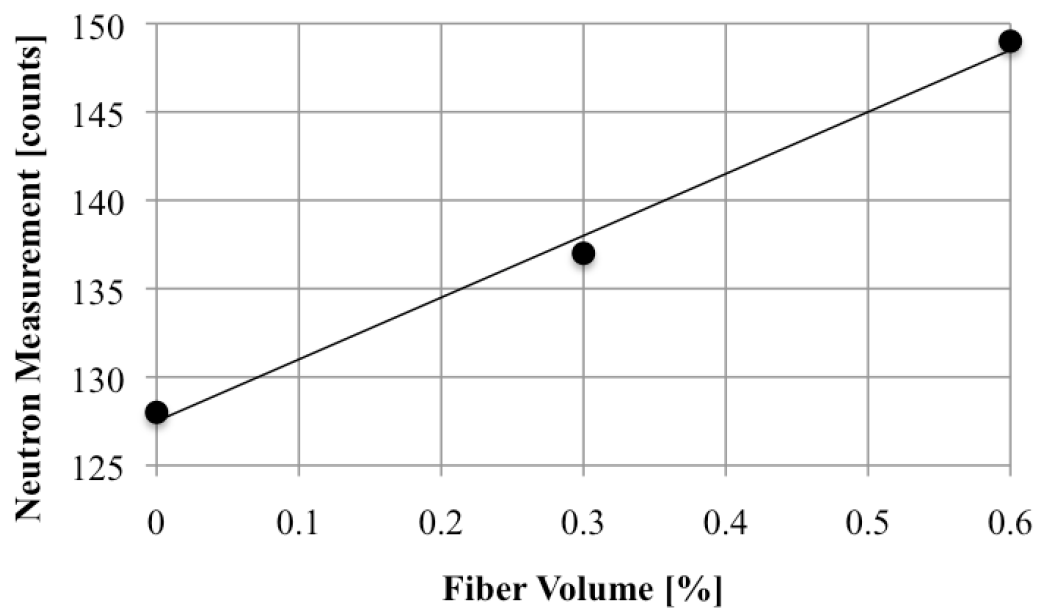
\includegraphics[width=.9\linewidth]{fig1.png}
\caption{Neutron Measurements and Linear Regression
of Laboratory Specimens.}
\label{fig:neutron}
\end{figure}

\subsection{Field Measurement \#1 and Results}
An existing 120 meter concrete pavement section with and without fibers was tested to examine the prediction capability of the nuclear gauge in the field. This pavement test section had two measurements done on the concrete with an asphalt base while three measurements were taken on a granular base layer as noted in Table \ref{tab:field1}. Ottawa sand was used beneath the gauge to level the gauge relative to the pavement surface.

\begin{table}%[tbhp]
\centering
\caption{Field Pavement Characteristics}
\label{tab:field1}
\begin{tabular}{rccc}
\multicolumn{1}{c}{Specimen ID} & Fibers? & Base Material & \begin{tabular}[c]{@{}c@{}}Pavement Thickness\\ {[}cm{]}\end{tabular} \\
\midrule
1-1 & N & Asphalt & 10.2 \\
1-2 & N & Asphalt & 15.2 \\
1-3 & N & Granular & 15.2 \\
1-4 & N & Granular & 20.3 \\
1-5 and 1-6 & Y & Granular & 8.9 \\
2-1 & N & -- & 15.2 \\
2-2 & Y & -- & 15.2 \\
2-3 & N & -- & 30.5 \\
2-4 & Y & -- & 30.5\\
\bottomrule
\end{tabular}
\end{table}

The initial results from the first field test section revealed a limiting factor in using the gauge for polymer fiber measurements. Table \ref{tab:field2} shows the data collected from the field concrete slabs revealed an opposite trend as what was expected based on the laboratory measurements. As noted in the Table 5, the depth of penetration is approximately 25 cm for the laboratory specimens and therefore it is expected the neutron count will be affected by the base layer beneath in the concrete slab in the field for these sections since they are all under 20 cm. For this current gauge configuration, there appears to be a required minimum pavement thickness needed to ensure that only the concrete volume is being measured and not the base layer beneath.

\begin{table*}[t]%[tbhp]
\caption{Neutron Measurements of Field \#1}
\label{tab:field2}
\centering
\begin{tabular}{rcccccc}
Specimen ID & 1-1 & 1-2 & 1-3 & 1-4 & 1-5\footnotemark[1] & 1-6\footnotemark[1] \\
\midrule
Thickness {[}cm{]} & 10.2 & 15.2 & 15.2 & 20.3 & 8.9 & 8.9 \\
Base Material & Asphalt & Asphalt & Granular & Granular & Granular & Granular \\
Average {[}counts{]} & 234 & 233 & 218 & 215 & 202 & 203 \\
St. Dev. {[}counts{]} & 6 & 4 & 9 & 5 & 4 & 7 \\
Coeff. of Var. & 2.6\% & 1.9\% & 4.0\% & 2.1\% & 1.8\% & 3.3\%\\
\bottomrule
\end{tabular}
%\begin{flushleft}
\footnotesize \footnotemark[1]These sections had fibers present.
%\end{flushleft}
\end{table*}


Specimens 1-1 and 1-2 had the highest neutron count. This is due to the significant amounts of hydrogen and carbon present in the asphalt base layer underneath the plain concrete slabs. Table 5 showed the neutrons penetrated about 7.6 and 12.7 cm into the asphalt layer and were easily thermalized as noted by the higher neutron count for specimens 1-1 and 1-2. The granular sections, 1-3 and 1-4, had significantly lower neutron counts as the base layer had less moisture and was not comprised of other significant neutron thermalizers. Ironically, the slab sections with fibers, 1-5 and 1-6, had the lowest neutron count readings. The factors affecting these particular measurements were the thickness of the section, fiber content resolution relative to other thermalizing sources, and base layer material and condition. The non-fiber sections on granular base were 15.2 and 20.3 cm thick while the fiber sections are only 8.9 cm thick with 0.4\% fibers. In general, it is possible that there may not be sufficient neutron thermalizers (e.g. polymer fibers) present to statistically affect the neutron count. This testing verified that with the current gauge sensor arrangement, thickness of the concrete layer, and amount of fibers, an accurate reading of fiber content is not possible.

\subsection{Field Measurements \#2 and Results}
A second field investigation on a different set of slab specimens was conducted because of conflicting results from the first field measurements. The slab specimens were 0.9 meters wide, 1.83 meters long, and 15.2 cm thick. Since it was known that 15.2 cm slab thickness was not sufficient to prevent neutrons from penetrating completely through the slab, two identical slabs, e.g., 2-3 and 2-4, were stacked on top of one another. This did create a potential for air pockets to be present at the interface. To determine if an air gap between the slabs would affect the gauge reading, a set of slabs, 2-1 and 2-2, were tested without stacking (Figure \ref{fig:neutron2} Table \ref{tab:penetrate}).

\begin{figure}%[tbhp]
\centering
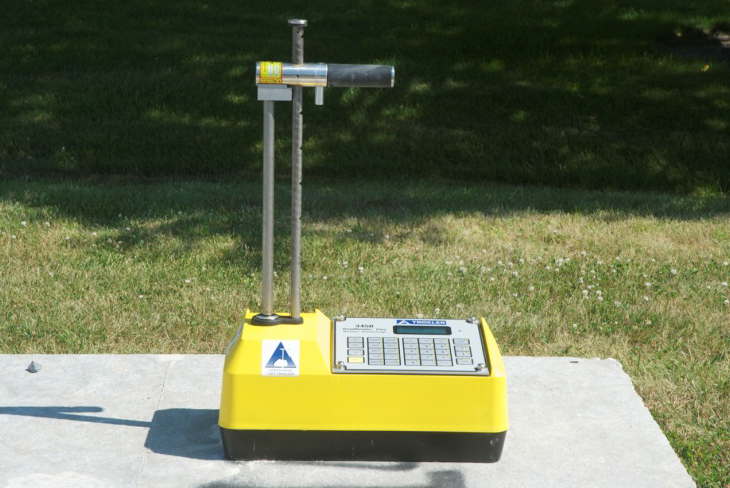
\includegraphics[width=.9\linewidth]{fig2.png}
\caption{Nuclear Density Gauge on Field Specimen 2-1.}
\label{fig:neutron2}
\end{figure}

With the knowledge of the first field test series, the second field test measurements, shown in Table \ref{tab:field3}, provided data that followed the trend of the laboratory specimen tests. The concrete slab specimens with fibers exhibited a higher neutron count. The measured fiber content was estimated by Eq. \ref{eq:linfit} and the neutron count. Because the laboratory and field concrete specimens had similar proportions and constituents, the slope of the field specimen measurements was assumed to be the same as the laboratory specimens. However, in practice, the gauge would need to be calibrated to the particular mix being used. To calibrate the offset of Eq. \ref{eq:linfit} to the particular mix, the equation was solved for the known state of 0\% fibers. The actual fiber content was verified by cutting samples out of the slab specimens and breaking them apart to weigh the fibers. Knowing the specific gravity of the fibers, the volume percentage could then be calculated.

\begin{table}%[tbhp]
\centering
\caption{Neutron Measurements of Field \#2}
\label{tab:field3}
\begin{tabular}{rcccc}
Specimen ID & 2-1 & 2-2 & 2-3 & 2-4 \\
\midrule
Thickness {[}in{]} & 15.2 & 15.2 & 30.5 & 30.5 \\
Average {[}counts{]} & 255 & 262 & 207 & 221 \\
St. Dev. {[}counts{]} & 9 & 4 & 5 & 5 \\
Coeff. of Var. & 3.5\% & 1.5\% & 2.4\% & 2.3\% \\
Measured Fiber Content & -- & 0.20\% & -- & 0.40\% \\
Actual Fiber Content & -- & 0.35\% & -- & 0.38\%\\
\bottomrule
\end{tabular}
\end{table}

The 15.2 cm specimen with fibers (2-2) significantly under predicted the fiber content present and the gauge measurement had a 42.9\% error when compared to the actual value. The fact that the neutrons penetrated through the slab into the support layer underneath explains the low neutron count. When the thickness was doubled to 30.5 cm, the neutron readings proved more reliable. The gauge measured the fiber content at 0.40\% while the true fiber content was 0.38\%, a 5.3\% error. This result, along with the laboratory specimen results, seems to indicate that a minimum thickness of 30 cm is required to obtain consistent and accurate measurements with the current gauge sensor layout. Therefore, a thick FRC slab in the field (> 30cm) is currently required to accurately assess the polymer fiber content with existing nuclear gage equipment. However, this limitation can be overcome if the source and detector positions could be optimally spaced to accommodate a thinner slab and determine near surface neutron count.

\section{Conclusions}
This study has shown that a nuclear density gauge can be useful tool for determining the polymer fiber content of a hardened concrete pavement. The process first involves taking a calibration measurement on a concrete section without fibers. Once the equation is calibrated to the particular concrete pavement involved, the gauge can be used to measure sections with polymer fibers. The thickness of the pavement is crucial to obtaining a proper measurement. It appears that a minimum thickness of 30 cm is needed to ensure that the neutrons do not penetrate into the base layer and produce erratic readings with the current setup. Measurements on a 30 cm thick concrete slab yielded a fiber content with only 5.3\% error. It is theoretically possible to significantly reduce the required slab thickness by adding an additional sensor and spacing them differently. It is also important to ensure that readings are taken relatively quickly to ensure the pavement is at a constant moisture state (i.e. not several days apart).

\acknow{The authors acknowledge the support from the National Science Foundation (NSF) through Grant CMMI \#0800805. The authors would also like to thank Ken Brown and Robyn Myers of Troxler Electronic Laboratories for their product support and technical assistance. The contents of this paper reflect the views of the authors, who are responsible for the accuracy of the data and facts presented herein.}

\showacknow % Display the acknowledgements section

% Bibliography
\bibliography{export.bib}

\end{document}